\section{Solucion}
\subsection{Objetivo}
\begin{frame}[shrink]
  \frametitle{Objetivo}
  Como respuesta a la situación actual, se define el siguiente objetivo:
  \begin{block}{Objetivo}
    Construir una solución de software libre con capacidades de WAF y aceleración SSL/TLS, que sea  fácilmente desplegable y que minimice el esfuerzo y el impacto que dicha
    solución tiene sobre la plataforma web actual o futura.
    \par También debe ser fácilmente adaptable a diferentes necesidades y entornos.
  \end{block}
\end{frame}

\subsection{Diseño}
\begin{frame}[shrink]
  \frametitle{Diseño}
  \begin{figure}
    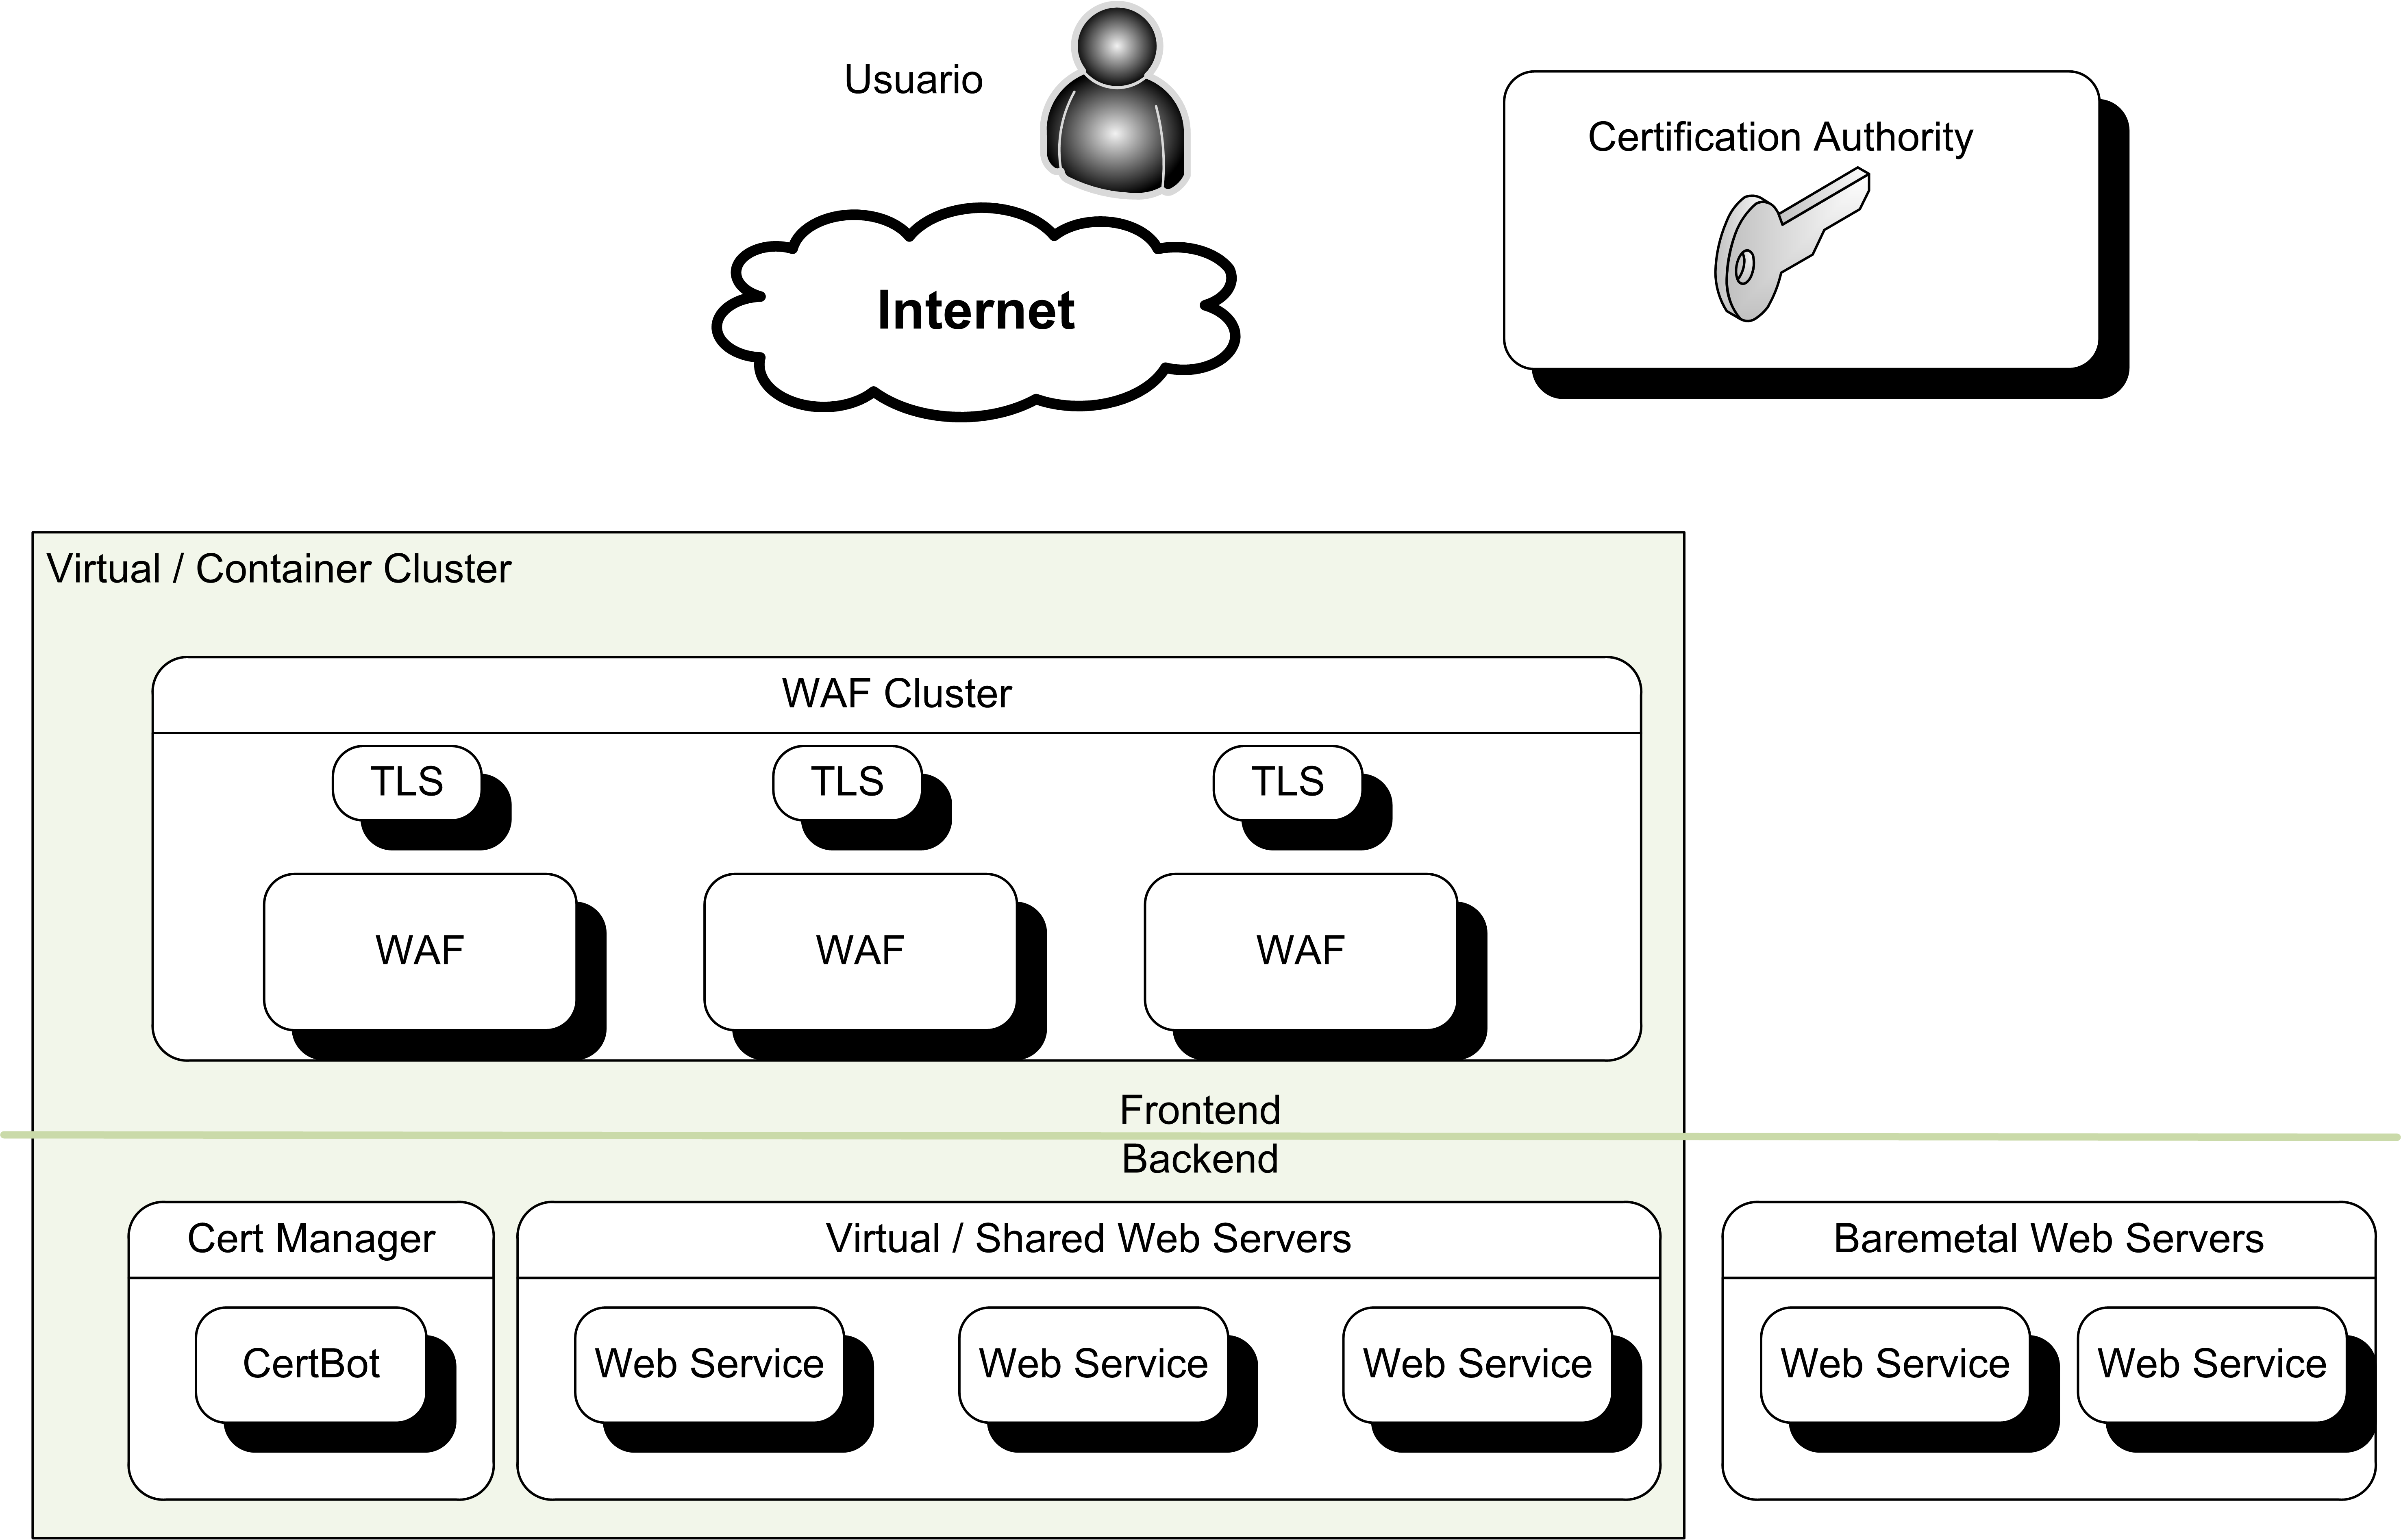
\includegraphics[width=0.9\textwidth]{fig/Diagram_HLD}
    \caption{\small{Diseño a alto nivel de la solución}}
  \end{figure}
\end{frame}

\begin{frame}[shrink]
  \frametitle{Componentes del WAF}
  \begin{figure}
    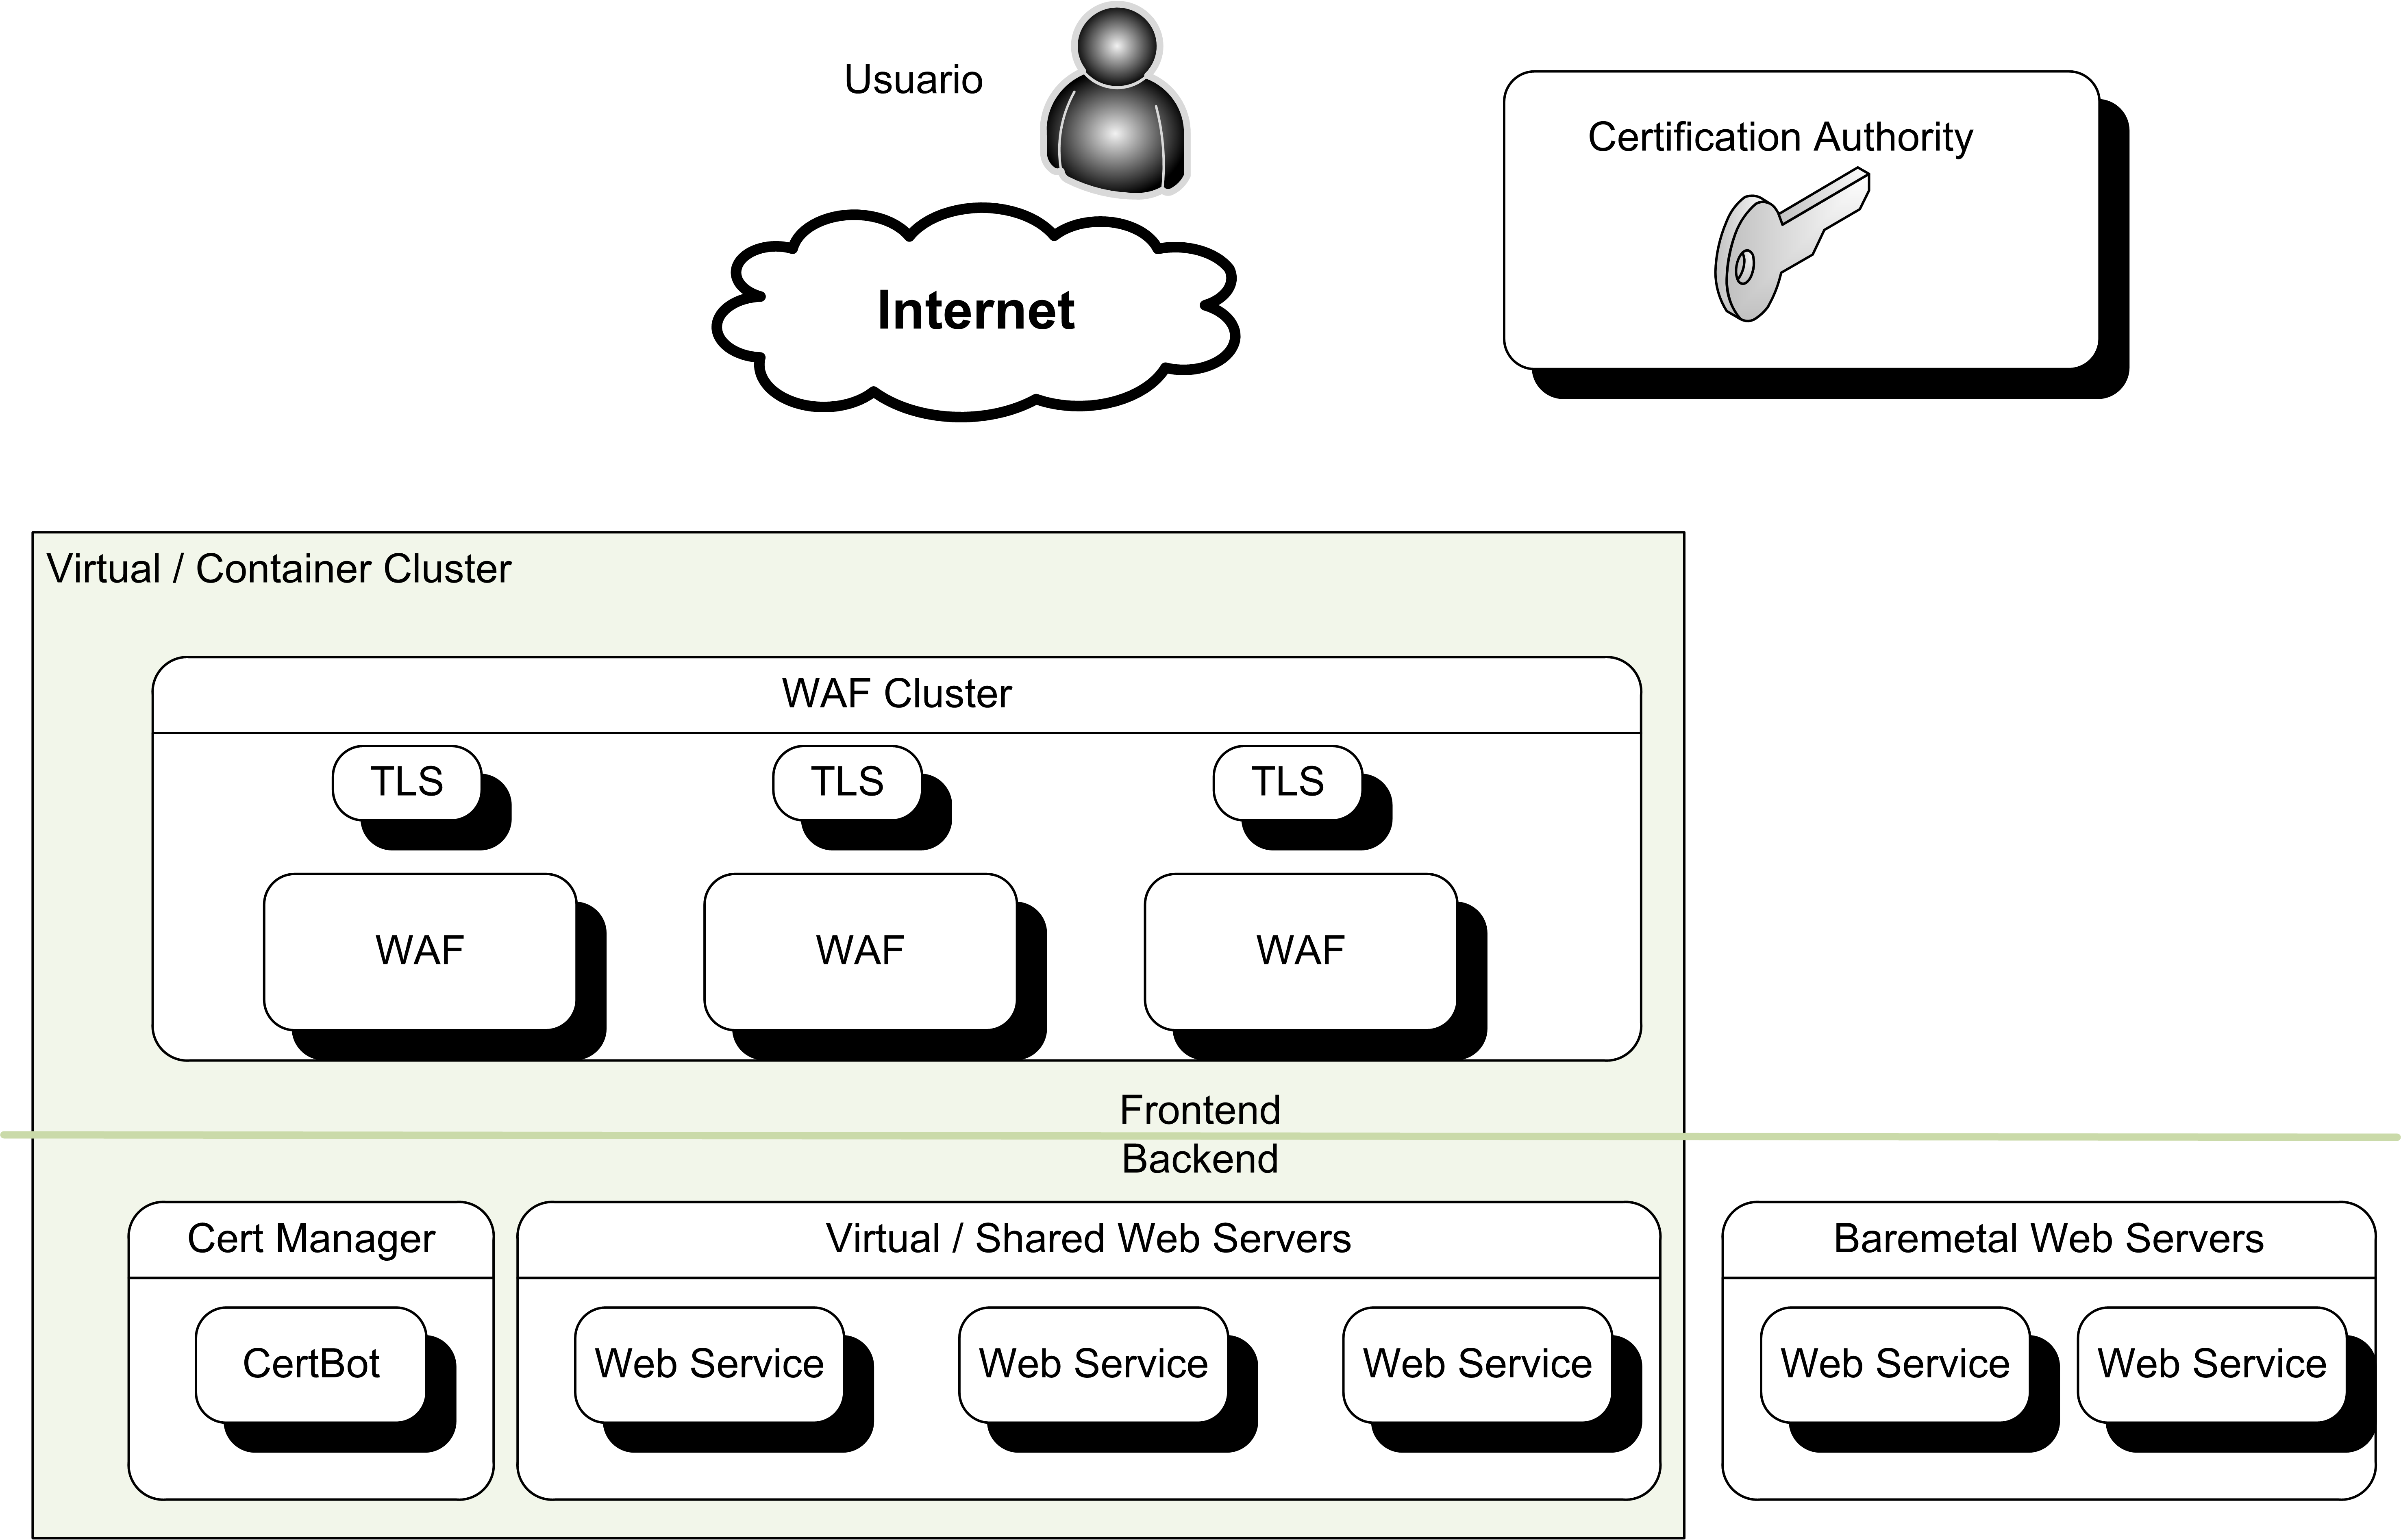
\includegraphics[width=0.9\textwidth]{fig/Diagram_HLD}
    \caption{\small{Diseño a alto nivel de la solución}}
  \end{figure}
\end{frame}

\begin{frame}[shrink]
  \frametitle{Componentes}
  \par Componentes de la solución:
  \begin{tabular}{ l c }
      \acrlong{waf}                                               & \parbox[c]{5em}{
\includegraphics[width=.30\textwidth,height=3cm,keepaspectratio]{fig/ModSecurityLogo}} \\
      Software criptográfico                                      & \parbox[c]{5em}{
\includegraphics[width=.30\textwidth,height=3cm,keepaspectratio]{OpenSSL_logo}} \\
      virtualización (contenedores)                               & \parbox[c]{5em}{
\includegraphics[width=.30\textwidth,height=3cm,keepaspectratio]{fig/DockerLogo}} \\
      Automatización y orquestación.                              & \parbox[c]{5em}{
\includegraphics[width=.30\textwidth,height=3cm,keepaspectratio]{fig/KubernetesLogo}} \\
      Gestión de certificados.                                    & \parbox[c]{5em}{
\includegraphics[width=.30\textwidth,height=3cm,keepaspectratio]{fig/LetsEncryptLogo}} \\
      Políticas y controles de seguridad.                         & \parbox[c]{5em}{
\includegraphics[width=.30\textwidth,height=3cm,keepaspectratio]{fig/OWASPCRSLogo}} \\
    \end{tabular}
\end{frame}


\subsection{Arquitectura}
\begin{frame}[shrink]
  \frametitle{Arquitectura. Gestión de certificados}
  \begin{figure}
    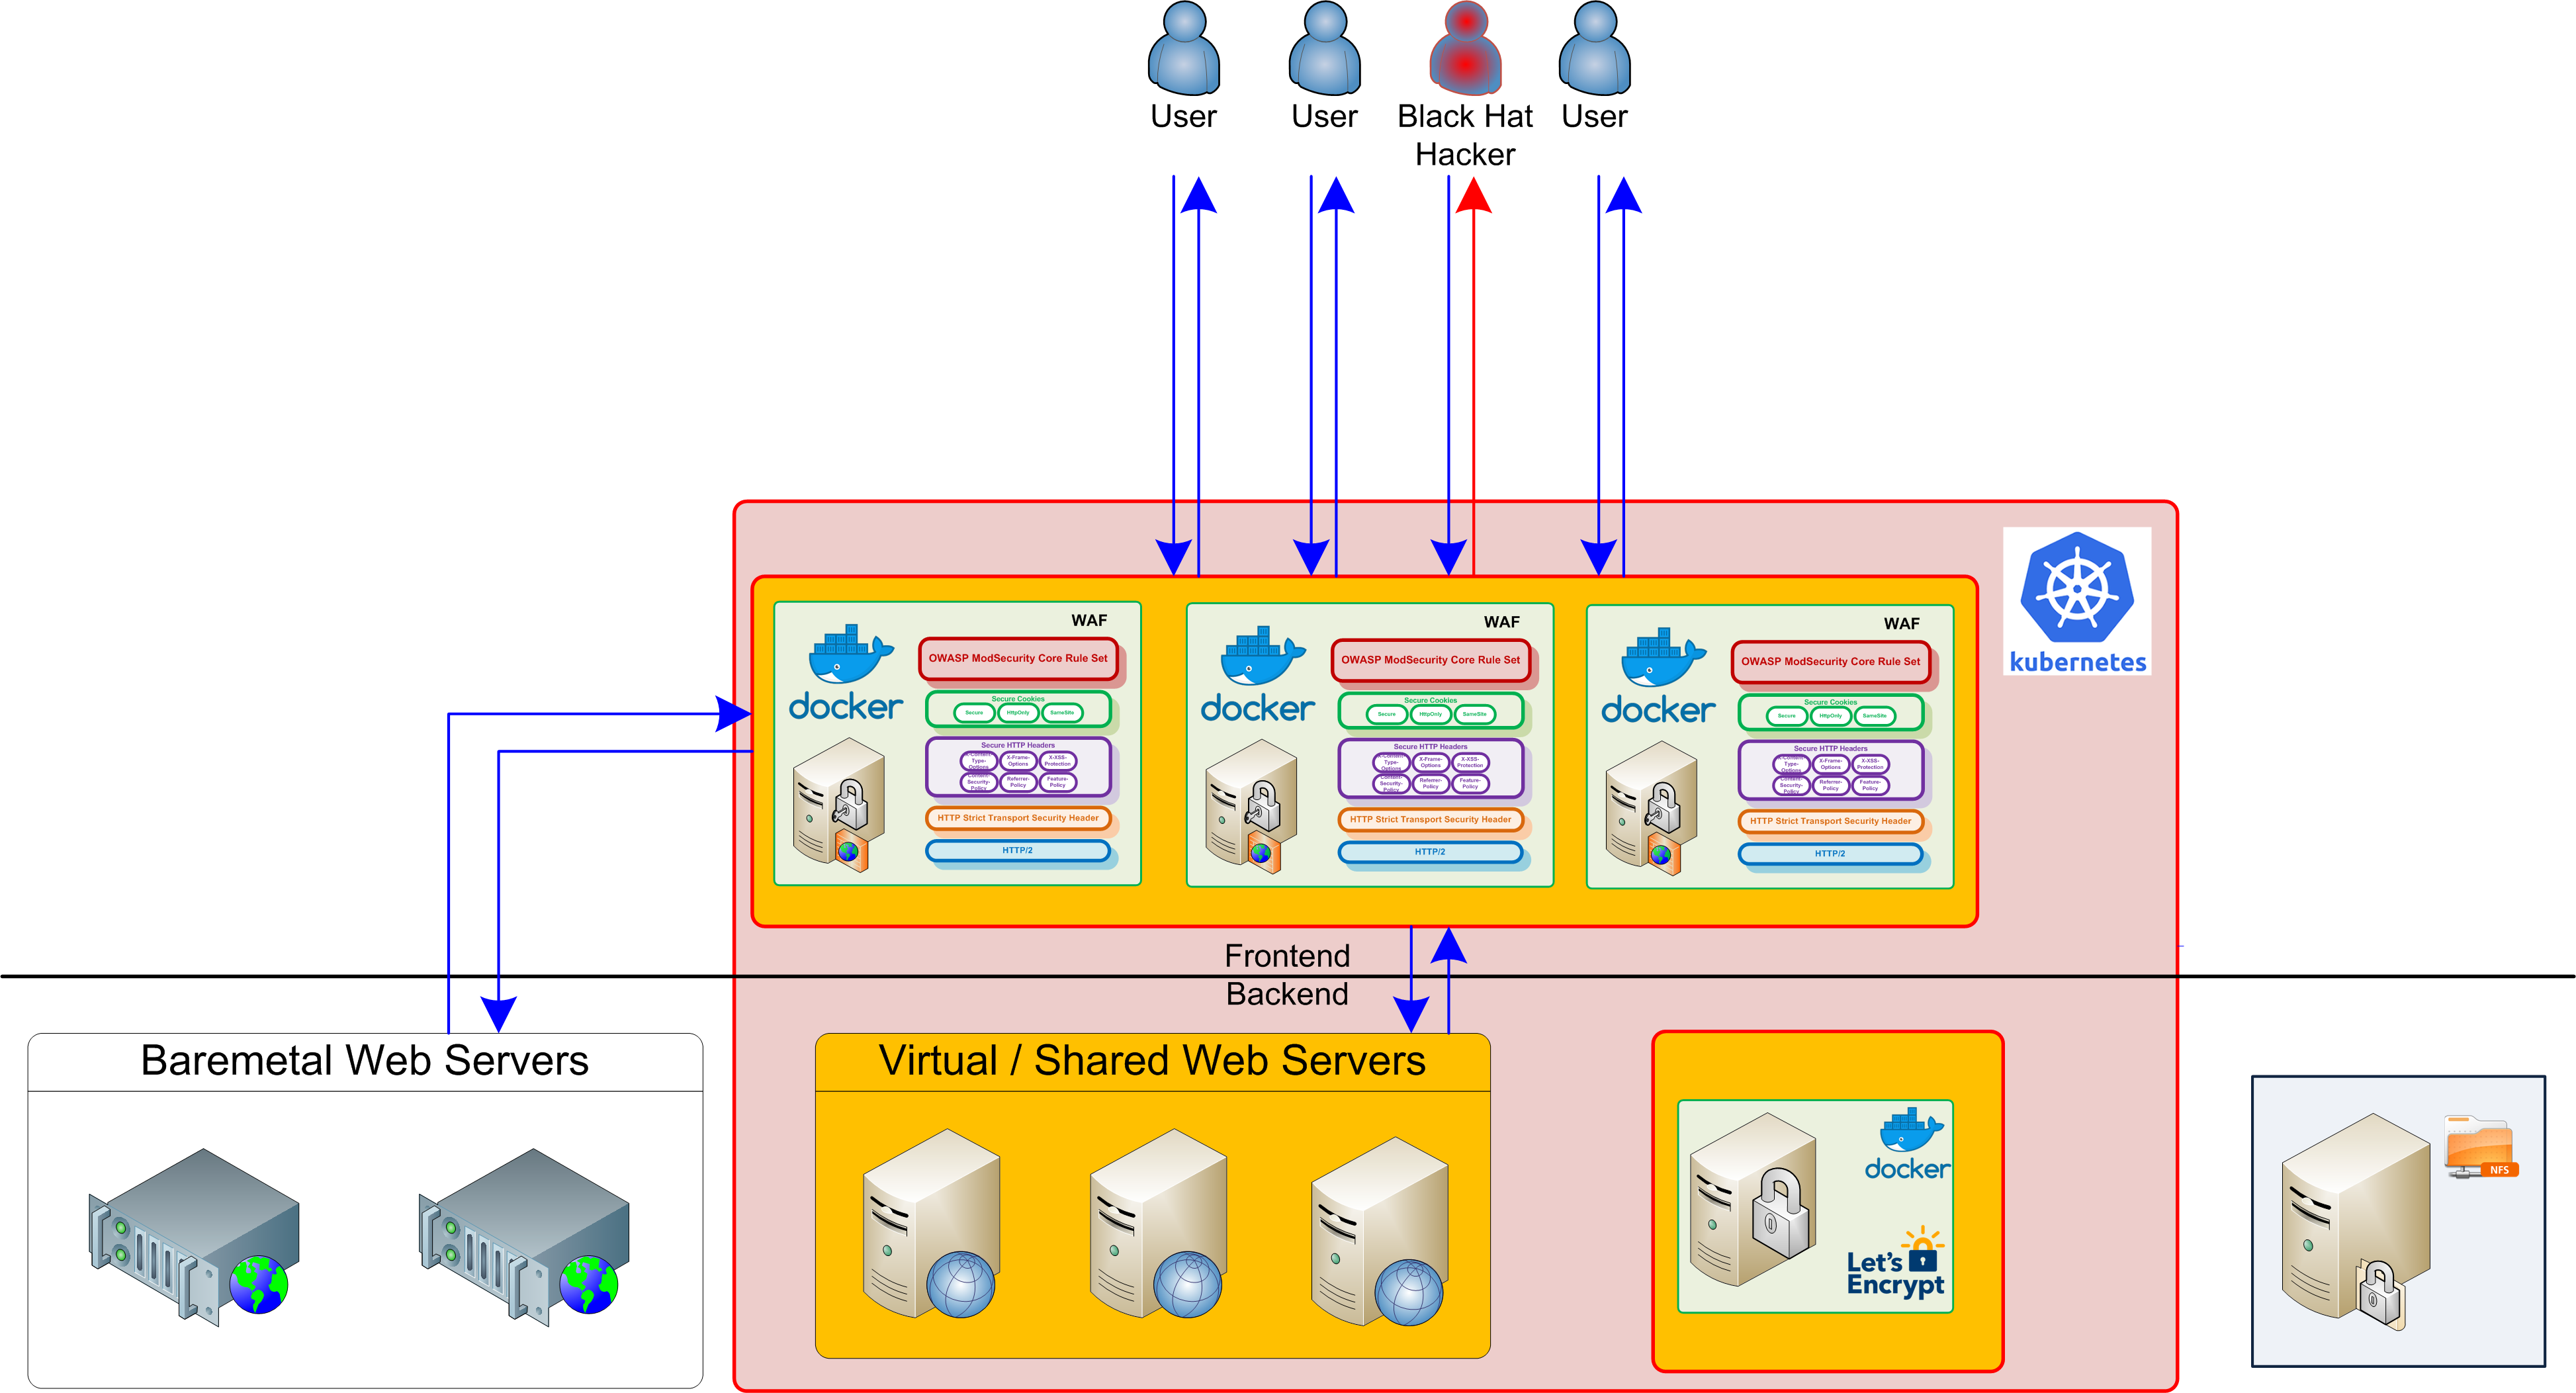
\includegraphics[width=0.9\textwidth]{fig/Diagram_HTTP_Services}
  \end{figure}
\end{frame}

\begin{frame}[shrink]
  \frametitle{Arquitectura. Peticiones HTTP/HTTPS}
  \begin{figure}
    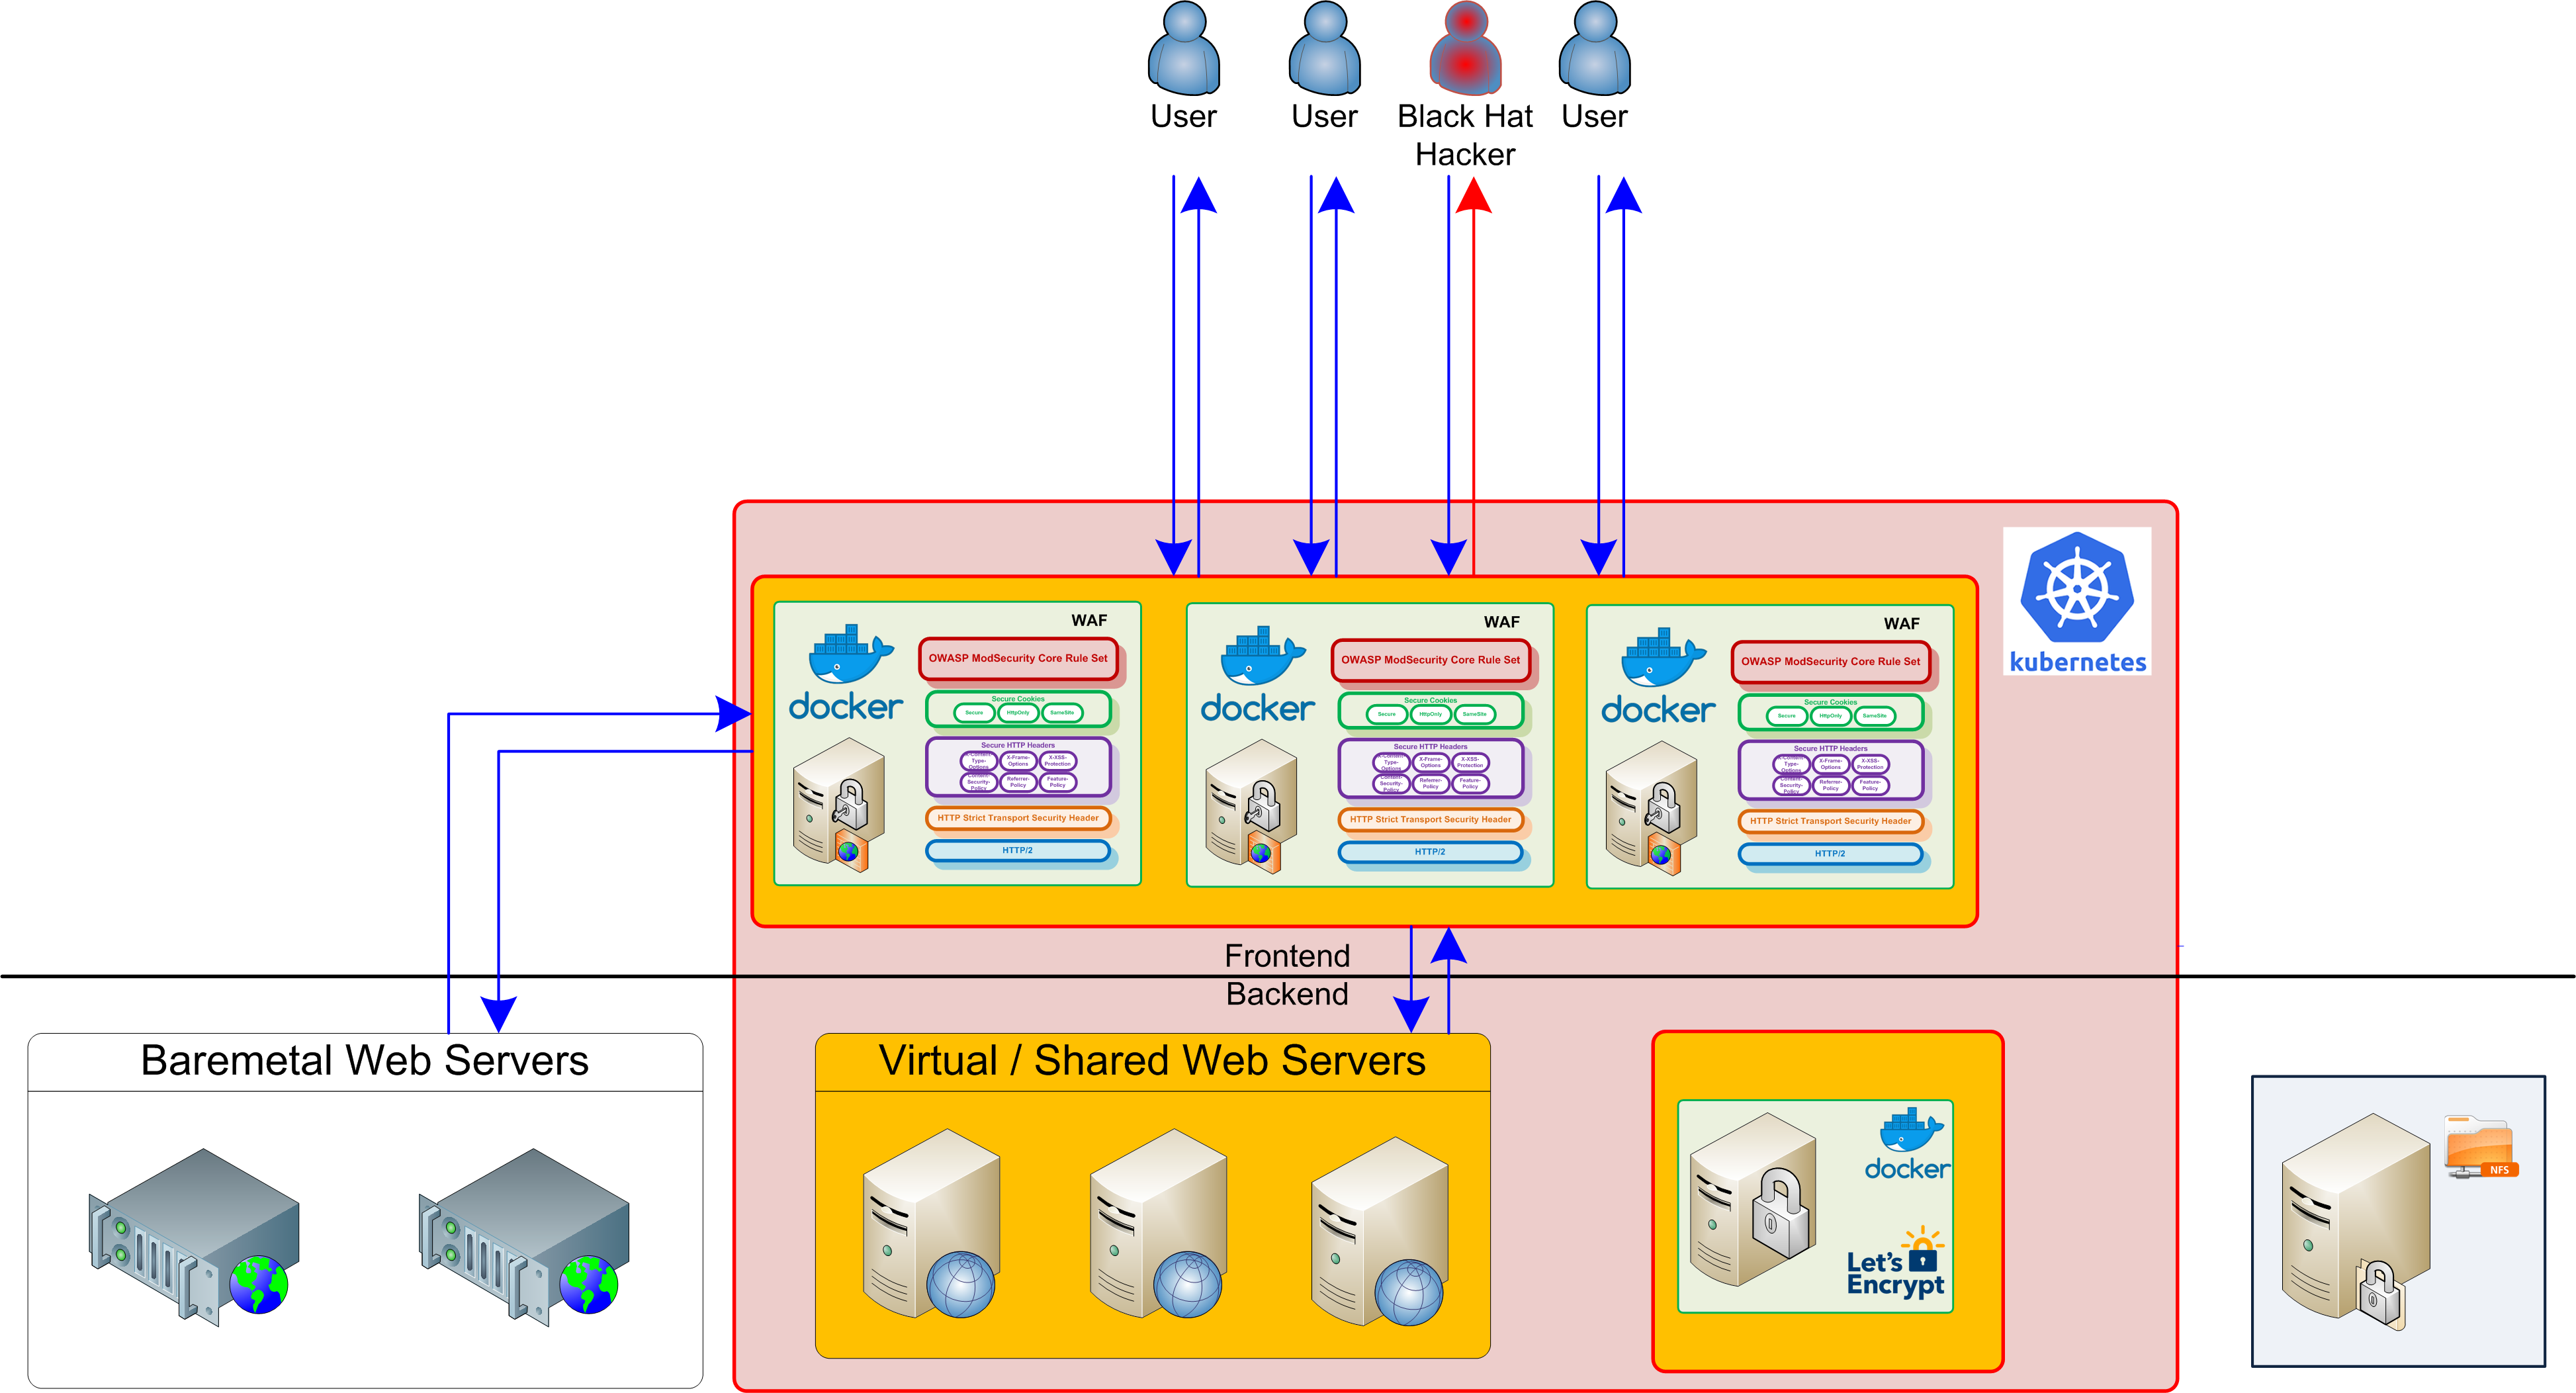
\includegraphics[width=0.9\textwidth]{fig/Diagram_HTTP_Services}
  \end{figure}
\end{frame}

